\documentclass[11pt]{article}
\usepackage[margin=1in]{geometry}
\usepackage{amsmath,amssymb,amsthm,mathtools}
\IfFileExists{lmodern.sty}{\usepackage{lmodern}}{}
\usepackage[expansion=false]{microtype}
\usepackage{booktabs,array,longtable}
\usepackage{enumitem}
\usepackage{xcolor}
\usepackage{tikz}
\usetikzlibrary{positioning,arrows.meta,fit,shapes.misc}
\usepackage[colorlinks=true,linkcolor=blue!50!black,citecolor=green!35!black,urlcolor=blue!50!black]{hyperref}
\usepackage[nameinlink]{cleveref}

\newtheorem{theorem}{Theorem}[section]
\newtheorem{proposition}[theorem]{Proposition}
\newtheorem{corollary}[theorem]{Corollary}
\theoremstyle{definition}
\newtheorem{definition}[theorem]{Definition}
\newtheorem{example}[theorem]{Example}
\theoremstyle{remark}
\newtheorem{remark}[theorem]{Remark}

\newcommand{\D}{\mathsf{D}}
\newcommand{\R}{\mathbb{R}}
\newcommand{\Z}{\mathbb{Z}}
\newcommand{\Cpl}{\operatorname{Cpl}}
\newcommand{\CP}{\mathbb{CP}}

\title{How the Programme Fits Together:\\ One Family of Polytopes, Many Models, and One Example Through Every Layer}
\author{Vinay K. Awasthi\\
Department of Applied Mathematics and Statistics\\
Johns Hopkins University\thanks{\texttt{check\_architecture.py} recomputes every number in \cref{sec:example,sec:deformation}. The other
results quoted here are proved or computed, with their own checks, in the papers cited.}}
\date{October 9, 2026, draft 1}

\begin{document}
\maketitle

\begin{abstract}
The programme consists of eight papers: a posterior tower, a categorical account of conditionals and couplings, a companion on coupling
polytopes, a paper on three layers of data, one on precise attribution, one on coupling algebras, one on bands of probabilities, and a note
on bridges to entropy and branes. This note explains how they fit together. The common object is not a single category or a single
geometric realization. It is the family of coupling polytopes, the fibres of the marginal map over the space of margins, together with its
stratification by walls and by the boundary of the simplex. Each paper puts one kind of structure on this family. Several mathematical
languages model it, and each sees something the others miss: linear programming, sheaves and descent, simplicial sets, cumulants and
$A_\infty$-structures, information geometry, toric and birational geometry, Floer theory, and stability conditions. Floer theory is one of
these models, not the privileged one. We test a proposed unification by deformation theory and find that it needs one correction. The
natural algebraic and complex-geometric objects are rigid: the gluing algebra is separable, the fibres are affine, and every $2\times3$ toric
surface has $H^1(T_X)=H^2(T_X)=0$. What moves with the margins is the symplectic class, which is the product coupling. Its deformation space
is the space of Kähler classes, cut into chambers by the secondary fan, and the bending, tearing and breaking of the bands paper are
movement inside a chamber, crossing a wall, and reaching the boundary of the effective cone. One $2\times3$ example is followed through every layer.
\end{abstract}

\tableofcontents

%=====================================================================
\section{Why this note}\label{sec:why}
%=====================================================================

A reader who meets the programme through one paper sees one structure: a tower of posteriors, a 2-cell, a polytope, a band, a brane. The
papers cite each other, but the reason they belong together is easy to miss. Two framings have been proposed to make it visible. One says
that Floer theory is only one of many possible realizations of the programme's structure. The other says that all the papers study one
deformation-theoretic object, a cotangent complex of the couplings. We keep the first and correct the second.

The plan is as follows. \Cref{sec:object} names the common object. \Cref{sec:papers} says what each paper does to it. \Cref{sec:models}
lists the models of the object and what each one sees and misses. \Cref{sec:deformation} tests the deformation-theoretic unification and
replaces it by a statement we can prove. \Cref{sec:example} follows one $2\times3$ example through every layer. \Cref{sec:status} separates
what is proved from what is computed and what is open.

%=====================================================================
\section{The common object}\label{sec:object}
%=====================================================================

Let $X$ and $Y$ be finite sets with $\lvert X\rvert=n$ and $\lvert Y\rvert=m$. The \emph{marginal map}
\[
M\colon\D(X\times Y)\longrightarrow\D(X)\times\D(Y),\qquad \pi\longmapsto(\pi_X,\pi_Y),
\]
sends a joint law to its two margins. Its fibre over $(f,g)$ is the coupling polytope $\Cpl(f,g)$, of dimension $(n-1)(m-1)$ when the margins
are positive. Its base, the space of margins, is cut by the \emph{walls} $f(I)=g(J)$, for nonempty proper $I\subset X$ and $J\subset Y$, into
\emph{chambers}, on which the combinatorial type of the fibre is constant \cite[Prop.~6.6]{Conditionals}. It is bounded by the faces of the
simplices, where a margin has a zero. With more than two variables the same picture holds for the map from a joint law to its marginals on a
cover, and then the fibre can be empty: that is contextuality \cite{AbramskyBrandenburger2011}.

\begin{center}
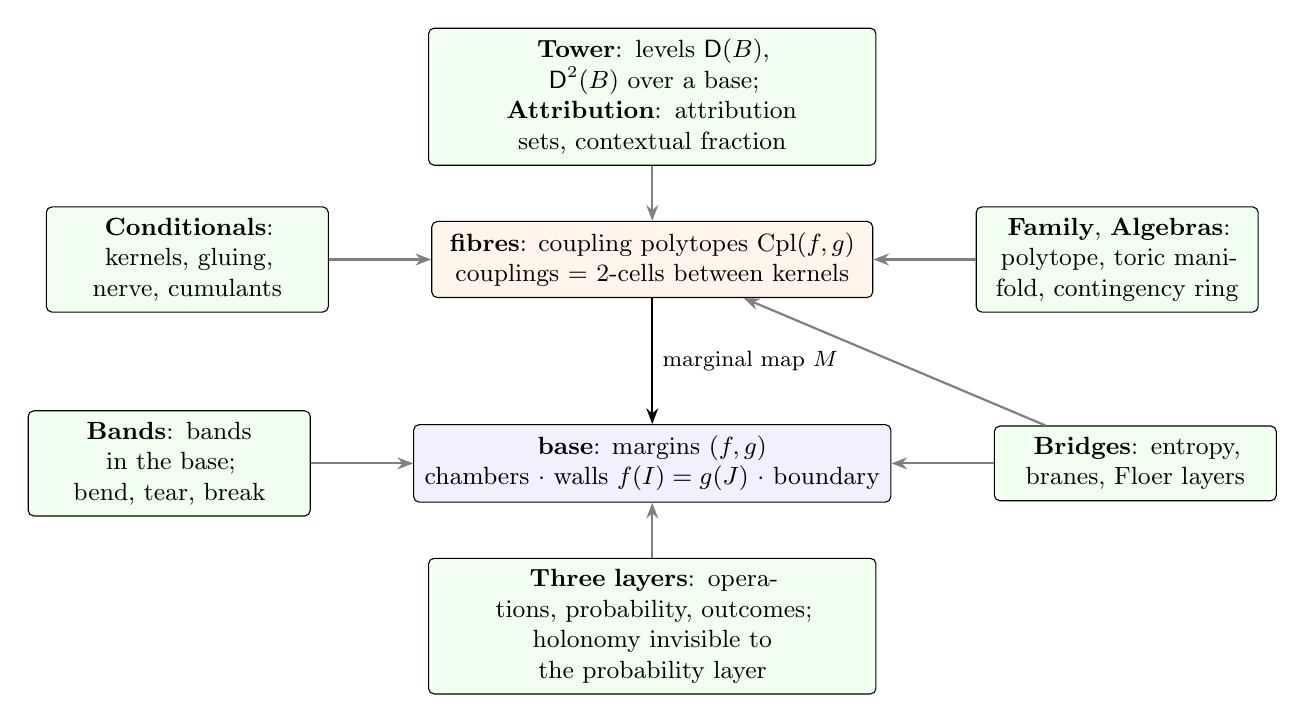
\begin{tikzpicture}[
  box/.style={draw, rounded corners=2pt, align=center, font=\small, inner sep=4pt, minimum height=0.9cm},
  lab/.style={font=\footnotesize, align=center},
  arr/.style={-{Stealth[length=2mm]}, thick}]
\node[box, fill=blue!6, minimum width=5.6cm] (base) {\textbf{base}: margins $(f,g)$\\ chambers $\cdot$ walls $f(I)=g(J)$ $\cdot$ boundary};
\node[box, fill=orange!8, minimum width=5.6cm, above=1.6cm of base] (fibre) {\textbf{fibres}: coupling polytopes $\Cpl(f,g)$\\ couplings = 2-cells between kernels};
\draw[arr] (fibre) -- node[right, lab] {marginal map $M$} (base);
\node[box, fill=green!6, left=1.3cm of base, text width=3.3cm] (bands) {\textbf{Bands}: bands in the base;\\ bend, tear, break};
\node[box, fill=green!6, left=1.3cm of fibre, text width=3.3cm] (cond) {\textbf{Conditionals}: kernels, gluing, nerve, cumulants};
\node[box, fill=green!6, right=1.3cm of fibre, text width=3.3cm] (fam) {\textbf{Family}, \textbf{Algebras}: polytope, toric manifold, contingency ring};
\node[box, fill=green!6, right=1.3cm of base, text width=3.3cm] (bri) {\textbf{Bridges}: entropy, branes, Floer layers};
\node[box, fill=green!6, above=0.7cm of fibre, minimum width=5.6cm, text width=5.4cm] (tower) {\textbf{Tower}: levels $\D(B)$, $\D^2(B)$ over a base;\\ \textbf{Attribution}: attribution sets, contextual fraction};
\node[box, fill=green!6, below=0.7cm of base, minimum width=5.6cm, text width=5.4cm] (tl) {\textbf{Three layers}: operations, probability, outcomes;\\ holonomy invisible to the probability layer};
\draw[arr, gray] (bands) -- (base); \draw[arr, gray] (cond) -- (fibre); \draw[arr, gray] (fam) -- (fibre); \draw[arr, gray] (bri) -- (base);
\draw[arr, gray] (bri) -- (fibre); \draw[arr, gray] (tower) -- (fibre); \draw[arr, gray] (tl) -- (base);
\end{tikzpicture}
\end{center}

Three features of this family carry most of the programme.
\begin{enumerate}[label=(\alph*),leftmargin=*]
\item \emph{Composition.} A coupling of $(f,g)$ and one of $(g,h)$ glue to a coupling of $(f,h)$. This is the vertical composition of
  2-cells \cite[\S2]{Conditionals}, it is strictly associative, and the whiskerings with stochastic kernels are not functorial.
\item \emph{Stratification.} The fibre changes combinatorial type only across walls, and loses dimension only at the boundary. This is
  what the bands paper calls tearing and breaking \cite[Thm.~3.3]{Bands}.
\item \emph{Positivity.} Laws are nonnegative. Most inequalities in the programme come from here: Fréchet bounds, the emptiness of
  fibres over cycles, the break margin, the tolerance of a band.
\end{enumerate}

%=====================================================================
\section{What each paper does}\label{sec:papers}
%=====================================================================

\begin{center}
\small
\begin{tabular}{p{2.6cm}p{5.6cm}p{6.6cm}}
\toprule
paper & acts on & main structures\\
\midrule
Tower \cite{Tower} & fibres over a fixed outcome base, at three levels & coherent contexts, a strict mixed distributive law, obstructions with certificates, transport along kernels\\
Conditionals \cite{Conditionals} & fibres and their composition & kernels as 1-cells, couplings as 2-cells, the graded shadow, the nerve $\D(Y^{\bullet+1})$, cumulants and the square-zero cone, toric realization\\
Family \cite{Family} & one fibre as a moment polytope & the $2\times3$ chambers and surfaces, Kähler class $=$ product coupling, disc potentials, stability conditions\\
Three layers \cite{ThreeLayers} & data seen through operations, probability, outcomes & holonomy, the contextual fraction on cycles, the separation of the three layers\\
Attribution \cite{Attribution} & polytopes of explanations & attribution sets, precision, mechanism reach, contextual fraction $=$ minimal unmodeled weight\\
Algebras \cite{Algebras} & the algebra of a fibre & the ring of contingency tables, the gluing algebra $A_f\cong\R\times M_{n-1}(\R)$\\
Bands \cite{Bands} & the base & bands, the three regimes, entropy on bands, the update monoid, limits, shards, horns and boundaries\\
Bridges \cite{Bridges} & maps out of the family & entropy and constraint branes, contextuality by default, toric branes, the modular Floer layers\\
\bottomrule
\end{tabular}
\end{center}

Read top to bottom, the table moves from the fibre over a single base point (Tower), through the structure of fibres and their composition
(Conditionals, Family, Algebras), to explanations and data (Attribution, Three layers), to the base and how it moves (Bands), and finally to
the maps from the whole family into other geometries (Bridges).

%=====================================================================
\section{Many models of one family}\label{sec:models}
%=====================================================================

Each language below models the family of \cref{sec:object}. None is complete, and the programme develops several of them side by side.
The right-hand column records what the model does not see, or, in the last rows, what has not been tested.

\begin{center}
\small
\begin{tabular}{p{2.4cm}p{4.7cm}p{3.1cm}p{4.3cm}}
\toprule
model & what it sees & where & what it misses\\
\midrule
linear programming & emptiness of fibres, contextual fraction, attribution sets, certificates & \cite{Attribution,Tower} & composition is only a set operation\\
sheaves and descent & compatible families on covers, global sections, contextuality by default & \cite{AbramskyBrandenburger2011,DzhafarovKujala2016}, \cite[\S4]{Bridges} & quantities: descent is yes or no until the contextual fraction is added\\
simplicial sets & the nerve $\D(Y^{\bullet+1})$, horn filling & \cite[\S4]{Conditionals}, \cite[Prop.~6.2]{Bands} & the Kan condition records failure, not its size\\
cumulants, $A_\infty$ & centred couplings, whiskering defects, the square-zero cone & \cite[\S5]{Conditionals} & cohomology keeps only the marginals; coupling data are homotopical\\
information geometry & Fisher metric, entropy, maximum-entropy laws, the entropy brane & \cite[\S\S2--3]{Bridges} & the walls: entropy is smooth across them\\
toric and birational geometry & moment polytopes, Kähler class, walls as variation of GIT & \cite[\S\S6, 10]{Conditionals}, \cite{Family} & positivity of the real points beyond the moment map\\
Floer theory & nonzero torus branes, leximin couplings, real locus & \cite[\S\S5, 8]{Bridges}, \cite[\S10.4]{Conditionals} & composition: gluing is not equivariantly induced \cite[Thm.~6.1]{Bridges}\\
stability conditions & central charges from $\omega_{f,g}$ & \cite{Family}, \cite[\S\S8, 10.3]{Conditionals} & hearts and the gluing condition are untested\\
dynamics & bands, tolerance, tear and break times, the update monoid & \cite{Bands} & higher structure, which lives on fibres\\
\bottomrule
\end{tabular}
\end{center}

Floer theory is one row of this table. Its strength is that it singles out couplings: for $2\times3$ margins, the nonzero torus branes sit
where cells are smallest and equal, the leximin coupling carries one in every computed case, and the maximum-entropy coupling carries none
when its smallest facet product $f_ig_j$ is unique \cite[Thm.~8.2]{Bridges}. Its weakness is composition, which it does not see. The sheaf and simplicial rows
see composition and its failure. The information-geometric row sees entropy but not the walls. No row is redundant.

A topos-theoretic model, in which contextuality is the failure of a global element of a presheaf, exists for quantum contextuality
\cite{IshamButterfield1998} and is close to the sheaf row. The programme has not developed it.

%=====================================================================
\section{Deformation theory: what it unifies and what it does not}\label{sec:deformation}
%=====================================================================

The proposal is that every paper studies one cotangent complex, with bending, tearing and breaking as its tangent space, its obstruction
space and its higher obstructions. Deformation theory has the right shape for a programme about perturbations, so the proposal deserves a
test. The test has three parts: what deforms, what its tangent and obstruction spaces are, and whether the regimes match them.

\subsection{The natural candidates are rigid}

\begin{proposition}[Rigidity]\label{prop:rigid}
\leavevmode
\begin{enumerate}[label=(\roman*)]
\item \emph{The fibre.} $\Cpl(f,g)$ is a polytope in an affine space. At a coupling in its relative interior, the first-order deformations
  with fixed margins are the matrices with zero row and column sums, a linear space of dimension $(n-1)(m-1)$, and there are no obstructions:
  every first-order deformation integrates to a line. At a boundary coupling, the directions that lower a zero cell do not integrate; that is
  positivity, not a cohomological obstruction.
\item \emph{The gluing algebra.} $A_f\cong\R\times M_{n-1}(\R)$ is separable, so its Hochschild cohomology vanishes above degree $0$
  \cite[Thm.~2.2]{Algebras}, \cite[Prop.~7.1]{Bridges}. It has no nontrivial deformations and no obstructions.
\item \emph{The complex structure.} Each of the five toric surfaces of $2\times3$ couplings has $H^1(X,T_X)=H^2(X,T_X)=0$. Its complex structure
  is rigid and unobstructed.
\end{enumerate}
\end{proposition}
\begin{proof}
(i) is linear algebra. (ii) is cited. (iii) The surfaces are del Pezzo, so $-K_X$ is ample, and by Serre duality and Akizuki--Nakano vanishing
$H^2(T_X)\cong H^0(\Omega^1_X\otimes K_X)^\vee=0$ \cite{AkizukiNakano1954}. Riemann--Roch for the rank-two bundle $T_X$ on a rational surface
gives $\chi(T_X)=2+K_X^2-e(X)=14-2r$ for a toric surface with $r$ rays. By Demazure, $h^0(T_X)=\dim\operatorname{Aut}(X)=2$ plus the number of
Demazure roots \cite{Demazure1970}. Counting roots gives $6,4,4,2,0$ for $\CP^2$, $\CP^1\times\CP^1$, $\mathbb F_1$, $\mathrm{Bl}_2\CP^2$ and
$\mathrm{Bl}_3\CP^2$, so $h^0=8,6,6,4,2=\chi(T_X)$ and $h^1(T_X)=0$. This agrees with Ilten's analysis of smooth toric surfaces
\cite{Ilten2009}. The counts are in \texttt{check\_architecture.py}.
\end{proof}

So the cotangent complexes of these three objects are trivial in the degrees that matter. (The proposition does not cover the quotients on
the walls, which are singular at flip walls, or the boundary fibres; these are where the programme's content sits.) By the proposal's own test, that "if the cotangent
complex is trivial, the programme is trivial", the programme would be trivial. It is not: it has walls, chambers, empty fibres and
nonzero contextual fractions. So the content of the programme does not live in these deformation spaces. The correspondence "bending $=T^1$,
tearing $=T^2$, breaking $=T^{\ge3}$" fails in particular. Bending is moving the margins within a chamber, which is the motion of the
Kähler class described in the next subsection, and tearing and breaking are not obstructions to extending a first-order deformation: they are changes of combinatorial type and of dimension, which happen at finite
distance \cite[Rem.~3.5]{Bands}.

\subsection{What does deform: the symplectic class}

The margins do not change the complex structure. They change the symplectic form. By \cite[Prop.~2.2]{Family}, the Kähler class of the
toric manifold of $\Cpl(f,g)$ is the product coupling read as divisor coefficients,
\[
[\omega_{f,g}]=\sum_{c=(i,j)\text{ facet}}f_ig_j\,[D_c]\in H^2(X;\R).
\]

\begin{proposition}[Margins as Kähler parameters]\label{prop:kahlermoduli}
For $2\times3$ couplings the map from margins $(f_1,g_1,g_2)$ to Kähler classes has rank $1,2,2,3,3$ on the chambers of type $\CP^2$,
$\CP^1\times\CP^1$, $\mathbb F_1$, $\mathrm{Bl}_2\CP^2$ and $\mathrm{Bl}_3\CP^2$, where $\dim H^2(X;\R)=1,2,2,3,4$. So the margins move the Kähler
class over an open subset of the Kähler cone, except for the degree-$6$ del Pezzo surface: there the six normals sum to zero, the sum of the
support numbers is $c_1\cdot[\omega]$, and on that chamber it equals $f_1+g_1+g_2+(g_3-f_1)=1$, so the margins sweep part of the hyperplane
$c_1\cdot[\omega]=1$ in the four-dimensional Kähler cone. Within a chamber the class moves in the ample cone of one surface; across a wall it
passes into the ample cone of a blow-up or blow-down; at the boundary of the space of margins it reaches the boundary of the effective cone.
\end{proposition}
\begin{proof}
The class is the vector of support numbers modulo linear functions; the ranks are computed in \texttt{check\_architecture.py}. The chamber
structure is that of variation of GIT \cite[Prop.~10.5]{Conditionals}, \cite{Thaddeus1996,DolgachevHu1998}, which for toric quotients is the
secondary fan \cite{GKZ1994,OdaPark1991}; a single wall crossing for $2\times3$ is one blow-up or blow-down \cite[Prop.~3.3]{Family}, \cite[Prop.~8.1]{Bridges}.
\end{proof}

This is the precise sense in which deformation theory organizes the programme. The deformation parameter is the symplectic class, its moduli
space is the Kähler cone of the family of surfaces glued along the walls of the secondary fan, and the three regimes are positions in that
space: inside an ample cone (bending), on a wall between two of them (tearing), and at the boundary of the effective cone (breaking).

\subsection{The Floer side has its own deformation space}

On the Floer side the deformation-theoretic statement is a theorem. Bulk deformations by classes $\mathfrak b$ deform the disc potential to
$\mathfrak{PO}_{\mathfrak b}$, and the Kodaira--Spencer map is a ring isomorphism
\[
QH_{\mathfrak b}(X;\Lambda_0)\cong\mathrm{Jac}(\mathfrak{PO}_{\mathfrak b})
\]
\cite[Thm.~1.1.1]{FOOO2016}. So the deformations of the potential are governed by quantum cohomology. For rational $2\times3$ margins the disc
potential is Morse, with as many critical points as the polygon has vertices \cite[Thm.~8.2]{Bridges}, so $QH(X;\Lambda)$, over the Novikov
field, is semisimple, a product of one copy of the field for each nonzero torus brane. For every $3\times3$ margin the potential is given by the
same uncorrected Laurent-polynomial formula, because the semi-Fano corrections vanish \cite[Thm.~8.4]{Bridges}; that it is Morse is shown for
one example \cite[Ex.~8.5]{Bridges}. Identifying this ring with the Hochschild cohomology of the Fukaya category, the object a cotangent-complex
proposal would point to, is the subject of \cite{AFOOO2026}. Either way it is a statement about one model, Floer theory, and not about the
whole family.

%=====================================================================
\section{One example through every layer}\label{sec:example}
%=====================================================================

Take $f=(0.4,0.6)$ and $g=(0.3,0.43,0.27)$. Write a coupling by its first-row cells $(\alpha_{11},\alpha_{12})$; the others follow from the
margins. Every number below is recomputed in \texttt{check\_architecture.py}.

\begin{center}
\small
\begin{longtable}{p{2.6cm}p{8.3cm}p{3.8cm}}
\toprule
layer & in the example & reference\\
\midrule
\endhead
fibre & $\Cpl(f,g)$ is a pentagon with vertices $(0,\frac{13}{100})$, $(0,\frac25)$, $(\frac{13}{100},0)$, $(\frac3{10},0)$, $(\frac3{10},\frac1{10})$ and area
$\frac{1331}{20000}$. Five cells can vanish; $\alpha_{22}\ge f_2+g_2-1=\frac3{100}$ cannot. & \cite[\S6]{Conditionals}, \cite[Prop.~8.1]{Bridges}\\
base & The wall values $f_1-g(J)$ are $\frac1{10},-\frac3{100},\frac{13}{100},-\frac{33}{100},-\frac{17}{100},-\frac3{10}$. The tear margin is $\frac3{100}$, at the wall
$f_1=g_2$, which is exactly where $\alpha_{22}$ could reach $0$; the break margin is $\frac{27}{100}$. & \cite[Thm.~3.2]{Bands}\\
bands & An elementwise band of half-width $\delta$ around $(f,g)$ meets no wall exactly when $\delta<\frac3{200}$. & \cite[Prop.~3.4]{Bands}\\
entropy & The maximum-entropy coupling is the product, $(\frac3{25},\frac{43}{250})$, with entropy $2.5256$ bits. The entropy brane meets the
conormal brane of the fibre there, transversally. & \cite[Thm.~3.1]{Bridges}\\
algebra & $A_f\cong\R\times\R$, which is semisimple, hence rigid. The ring of contingency tables of the lattice polytope $100\cdot\Cpl(f,g)$ is its
Ehrhart ring, with $X$ as its $\operatorname{Proj}$. & \cite[Thms.~2.2, 7.1]{Algebras}, \cite[Prop.~7.1]{Bridges}\\
toric & $X=\mathrm{Bl}_2\CP^2$, with invariant curves of self-intersection $0,-1,0,-1,-1$ on the cells $11,12,13,21,23$, and Kähler class
$\frac3{25}D_{11}+\frac{43}{250}D_{12}+\frac{27}{250}D_{13}+\frac9{50}D_{21}+\frac{81}{500}D_{23}$. The function $-\frac12H$ is an admissible symplectic potential.
$h^0(T_X)=4$, $h^1=h^2=0$. & \cite{Family}, \cite[Thm.~5.1]{Bridges}, \cref{prop:rigid}\\
crossing the wall & Moving $g_2$ below $f_1$ makes $\alpha_{22}$ a facet: the pentagon becomes a hexagon, $X$ is blown up to the degree-$6$ del Pezzo
surface, and one more vertex and one more nonzero brane appear. & \cite[Prop.~3.3]{Family}, \cite[Prop.~8.1, Thm.~8.2]{Bridges}\\
Floer & Five nonzero torus branes, all distinct: three over the leximin coupling $(\frac2{15},\frac2{15})$, where $\alpha_{11}=\alpha_{12}=\alpha_{13}=\frac2{15}$;
one over $(\frac{13}{100},\frac{13}{100})$, where $\alpha_{11}=\alpha_{12}=\alpha_{23}$; one over $(\frac15,\frac1{10})$, where $\alpha_{12}=\alpha_{13}=\alpha_{21}$.
None over the product coupling, whose smallest facet cell $\alpha_{13}=\frac{27}{250}$ is unique. & \cite[Thm.~8.2]{Bridges}\\
real locus & $X^{\R}=\#3\,\mathbb{RP}^2$, Euler characteristic $-1$, non-orientable; the three $(-1)$-curves give discs of Maslov index $1$, so its Floer
theory needs bounding cochains (open). & \cite[Prop.~8.6]{Bridges}\\
nerve & A single table has one context, so it is always compatible. Contextuality needs a cycle of contexts: three pairwise tables on three
variables, the boundary of a $2$-simplex, the smallest configuration that need not fill. & \cite[Prop.~4.5]{Conditionals}, \cite[Prop.~6.2(ii)]{Bands}\\
contextuality by default & If the same variable is measured in two contexts with different laws, the fibre condition is replaced by maximal
couplings of its copies. & \cite[\S4]{Bridges}\\
tower and attribution & Read as a claim about a joint law with these margins, the pentagon is the admissible set at level one; obstructions
and certificates come from linear programming; for a horn encoded as a level-one claim the secondary obstruction is at least twice the
contextual fraction, with equality when all compatible families are admissible. & \cite{Tower}, \cite[Thm.~11.2]{Conditionals}, \cite{Attribution}\\
three layers & What this example cannot show: holonomy of operations is invisible to the probability layer. & \cite{ThreeLayers}\\
\bottomrule
\end{longtable}
\end{center}

The example shows the division of labour. The polytope, its walls and its entropy are probability. The rigidity of $X$ and the motion of its
Kähler class are the deformation theory. The three couplings over which branes sit, and the absence of the maximum-entropy coupling among
them, are what the Floer model adds. The fact that one table can never be contextual, while three can, is what the sheaf and simplicial
models add.

%=====================================================================
\section{Status}\label{sec:status}
%=====================================================================

\begin{center}
\small
\begin{tabular}{p{7.2cm}p{2.2cm}p{5.4cm}}
\toprule
statement & status & where\\
\midrule
gluing is strictly associative; whiskering by stochastic kernels is not functorial & proved & \cite{Conditionals}\\
2-horns fill, $n$-horns can fail, the nerve is not Kan & proved & \cite[\S4]{Conditionals}, \cite[Prop.~6.2]{Bands}\\
contextual fraction $=$ minimal unmodeled weight & proved & \cite{Attribution}\\
coupling polytopes of nondegenerate margins are Delzant; Kähler class $=$ product coupling & proved & \cite[Thm.~6.4]{Conditionals}, \cite[Prop.~2.2]{Family}\\
walls are variation-of-GIT walls & proved & \cite[Prop.~10.5]{Conditionals}\\
compatibility is lost only through breaking & proved & \cite[Thm.~8.1]{Bands}\\
entropy brane meets the constraint brane once, transversally, when a positive law satisfies the constraint & proved & \cite[Thm.~3.1]{Bridges}\\
$2\times3$: Morse potential (rational margins), two kinds of brane (off finitely many planes), product coupling excluded (unique smallest
facet product) & proved & \cite[Thm.~8.2]{Bridges}\\
$3\times3$: semi-Fano, no disc-potential corrections & proved by computation over all chambers & \cite[Thm.~8.4]{Bridges}\\
natural algebraic and complex deformations are rigid; margins move the Kähler class & proved & \cref{prop:rigid,prop:kahlermoduli}\\
leximin coupling carries a brane & computed ($2970$ cases) & \cite[Thm.~8.2(iv)]{Bridges}\\
Floer theory of the real locus beyond monotone cases & open & \cite[\S8.4]{Bridges}\\
sheaf model of the entropy brane & open (one isotopy) & \cite[Prop.~8.7]{Bridges}\\
no torus-equivariant correspondence induces gluing by a non-constant stochastic kernel & proved (no-go) & \cite[Thm.~6.1]{Bridges}\\
a topos-theoretic model & not developed & \cite{IshamButterfield1998}\\
\bottomrule
\end{tabular}
\end{center}

\paragraph{How to read the programme.} Start with \cref{sec:object}. Then read the paper whose model is closest to the reader's own
field, using \cref{sec:models} to find it, and use the example of \cref{sec:example} as a dictionary between that paper and the others. A
statement proved in one model is a statement about the family; whether it transfers to another model is a separate question, and the
programme answers it only where the table above says so.

%=====================================================================
\section{Computational checks}\label{sec:code}
%=====================================================================

\texttt{check\_architecture.py} recomputes the example of \cref{sec:example} (the polygon, its area, the walls and margins, the band
tolerance, the product coupling and its entropy, the self-intersections and Kähler coefficients, the five brane positions with their
multiplicities and their distinctness), the Demazure-root counts and Euler characteristics of \cref{prop:rigid}, and the ranks of
\cref{prop:kahlermoduli}. It uses the exact routines of \cite[\S8]{Bridges}.

\begin{thebibliography}{99}

\bibitem{Algebras}
V.~K. Awasthi, Coupling algebras: gluing, the square-zero cone and the ring of contingency tables. Technical report, Johns
Hopkins University, October 2026. Draft 4.

\bibitem{Attribution}
V.~K. Awasthi, Precise attribution of model interventions: attribution sets, mechanism reach, path defects and gluing.
Technical report, Johns Hopkins University, October 2026. Draft 5.

\bibitem{Bands}
V.~K. Awasthi, Bands: perturbation, tearing and breaking of coupling structures, and the entropy of changing probabilities.
Technical report, Johns Hopkins University, October 2026. Draft 2.

\bibitem{Bridges}
V.~K. Awasthi, Bridges: from probability and entropy to branes, with worked examples. Technical note, Johns Hopkins University,
October 2026. Draft 4.

\bibitem{Conditionals}
V.~K. Awasthi, Conditionals, couplings and toric geometry: kernels, the coupling nerve, cumulants and a {F}ukaya
programme. Technical report, Johns Hopkins University, October 2026. Revised draft 4.

\bibitem{Family}
V.~K. Awasthi, Coupling polytopes and toric geometry: the $2\times3$ family, the square case, higher levels and stability.
Companion paper, Johns Hopkins University, October 2026.

\bibitem{ThreeLayers}
V.~K. Awasthi, Three layers of realisation: hierarchy recovery, holonomy, information, contextuality and categorical
dynamics. Technical report, Johns Hopkins University, revised October 2026. DOI: 10.13140/RG.2.2.24274.52163.

\bibitem{Tower}
V.~K. Awasthi, The three-level posterior tower: hierarchical {B}ayesian inference and mixed distributive laws.
Technical report, Johns Hopkins University, October 2026. Revised version 10.

\bibitem{AbramskyBrandenburger2011}
S.~Abramsky and A.~Brandenburger, The sheaf-theoretic structure of non-locality and contextuality. \emph{New J. Phys.}
\textbf{13} (2011), 113036.

\bibitem{AFOOO2026}
M.~Abouzaid, K.~Fukaya, Y.-G. Oh, H.~Ohta and K.~Ono, Quantum cohomology and split generation in Lagrangian Floer theory.
Preprint, arXiv:2606.12257, 2026.

\bibitem{AkizukiNakano1954}
Y.~Akizuki and S.~Nakano, Note on Kodaira--Spencer's proof of Lefschetz theorems. \emph{Proc. Japan Acad.} \textbf{30} (1954),
266--272.

\bibitem{Demazure1970}
M.~Demazure, Sous-groupes algébriques de rang maximum du groupe de Cremona. \emph{Ann. Sci. École Norm. Sup.} (4) \textbf{3} (1970),
507--588.

\bibitem{DolgachevHu1998}
I.~V. Dolgachev and Y.~Hu, Variation of geometric invariant theory quotients. \emph{Publ. Math. IHÉS} \textbf{87} (1998), 5--56.

\bibitem{DzhafarovKujala2016}
E.~N. Dzhafarov and J.~V. Kujala, Context-content systems of random variables: the Contextuality-by-Default theory.
\emph{J. Math. Psych.} \textbf{74} (2016), 11--33.

\bibitem{FOOO2016}
K.~Fukaya, Y.-G. Oh, H.~Ohta and K.~Ono, Lagrangian Floer theory and mirror symmetry on compact toric manifolds. \emph{Astérisque}
\textbf{376} (2016).

\bibitem{GKZ1994}
I.~M. Gelfand, M.~M. Kapranov and A.~V. Zelevinsky, \emph{Discriminants, Resultants, and Multidimensional Determinants}.
Birkhäuser, 1994.

\bibitem{Ilten2009}
N.~O. Ilten, Deformations of smooth toric surfaces. \emph{Manuscripta Math.} \textbf{134} (2011), 123--137; arXiv:0902.0529.

\bibitem{IshamButterfield1998}
C.~J. Isham and J.~Butterfield, A topos perspective on the Kochen--Specker theorem {I}: quantum states as generalized valuations.
\emph{Int. J. Theor. Phys.} \textbf{37} (1998), 2669--2733.

\bibitem{OdaPark1991}
T.~Oda and H.~S. Park, Linear Gale transforms and Gelfand--Kapranov--Zelevinskij decompositions. \emph{Tohoku Math. J.} \textbf{43}
(1991), 375--399.

\bibitem{Thaddeus1996}
M.~Thaddeus, Geometric invariant theory and flips. \emph{J. Amer. Math. Soc.} \textbf{9} (1996), 691--723.

\end{thebibliography}
\end{document}
